\pagestyle{kalinka}
\label{kalinka}

\pagebreak 

\begin{center}
\hspace*{-3.6cm}\raisebox{5cm}{\rotatebox[origin=t]{90}{\huge\textbf{Lançamento}}}
\hspace*{3.1cm}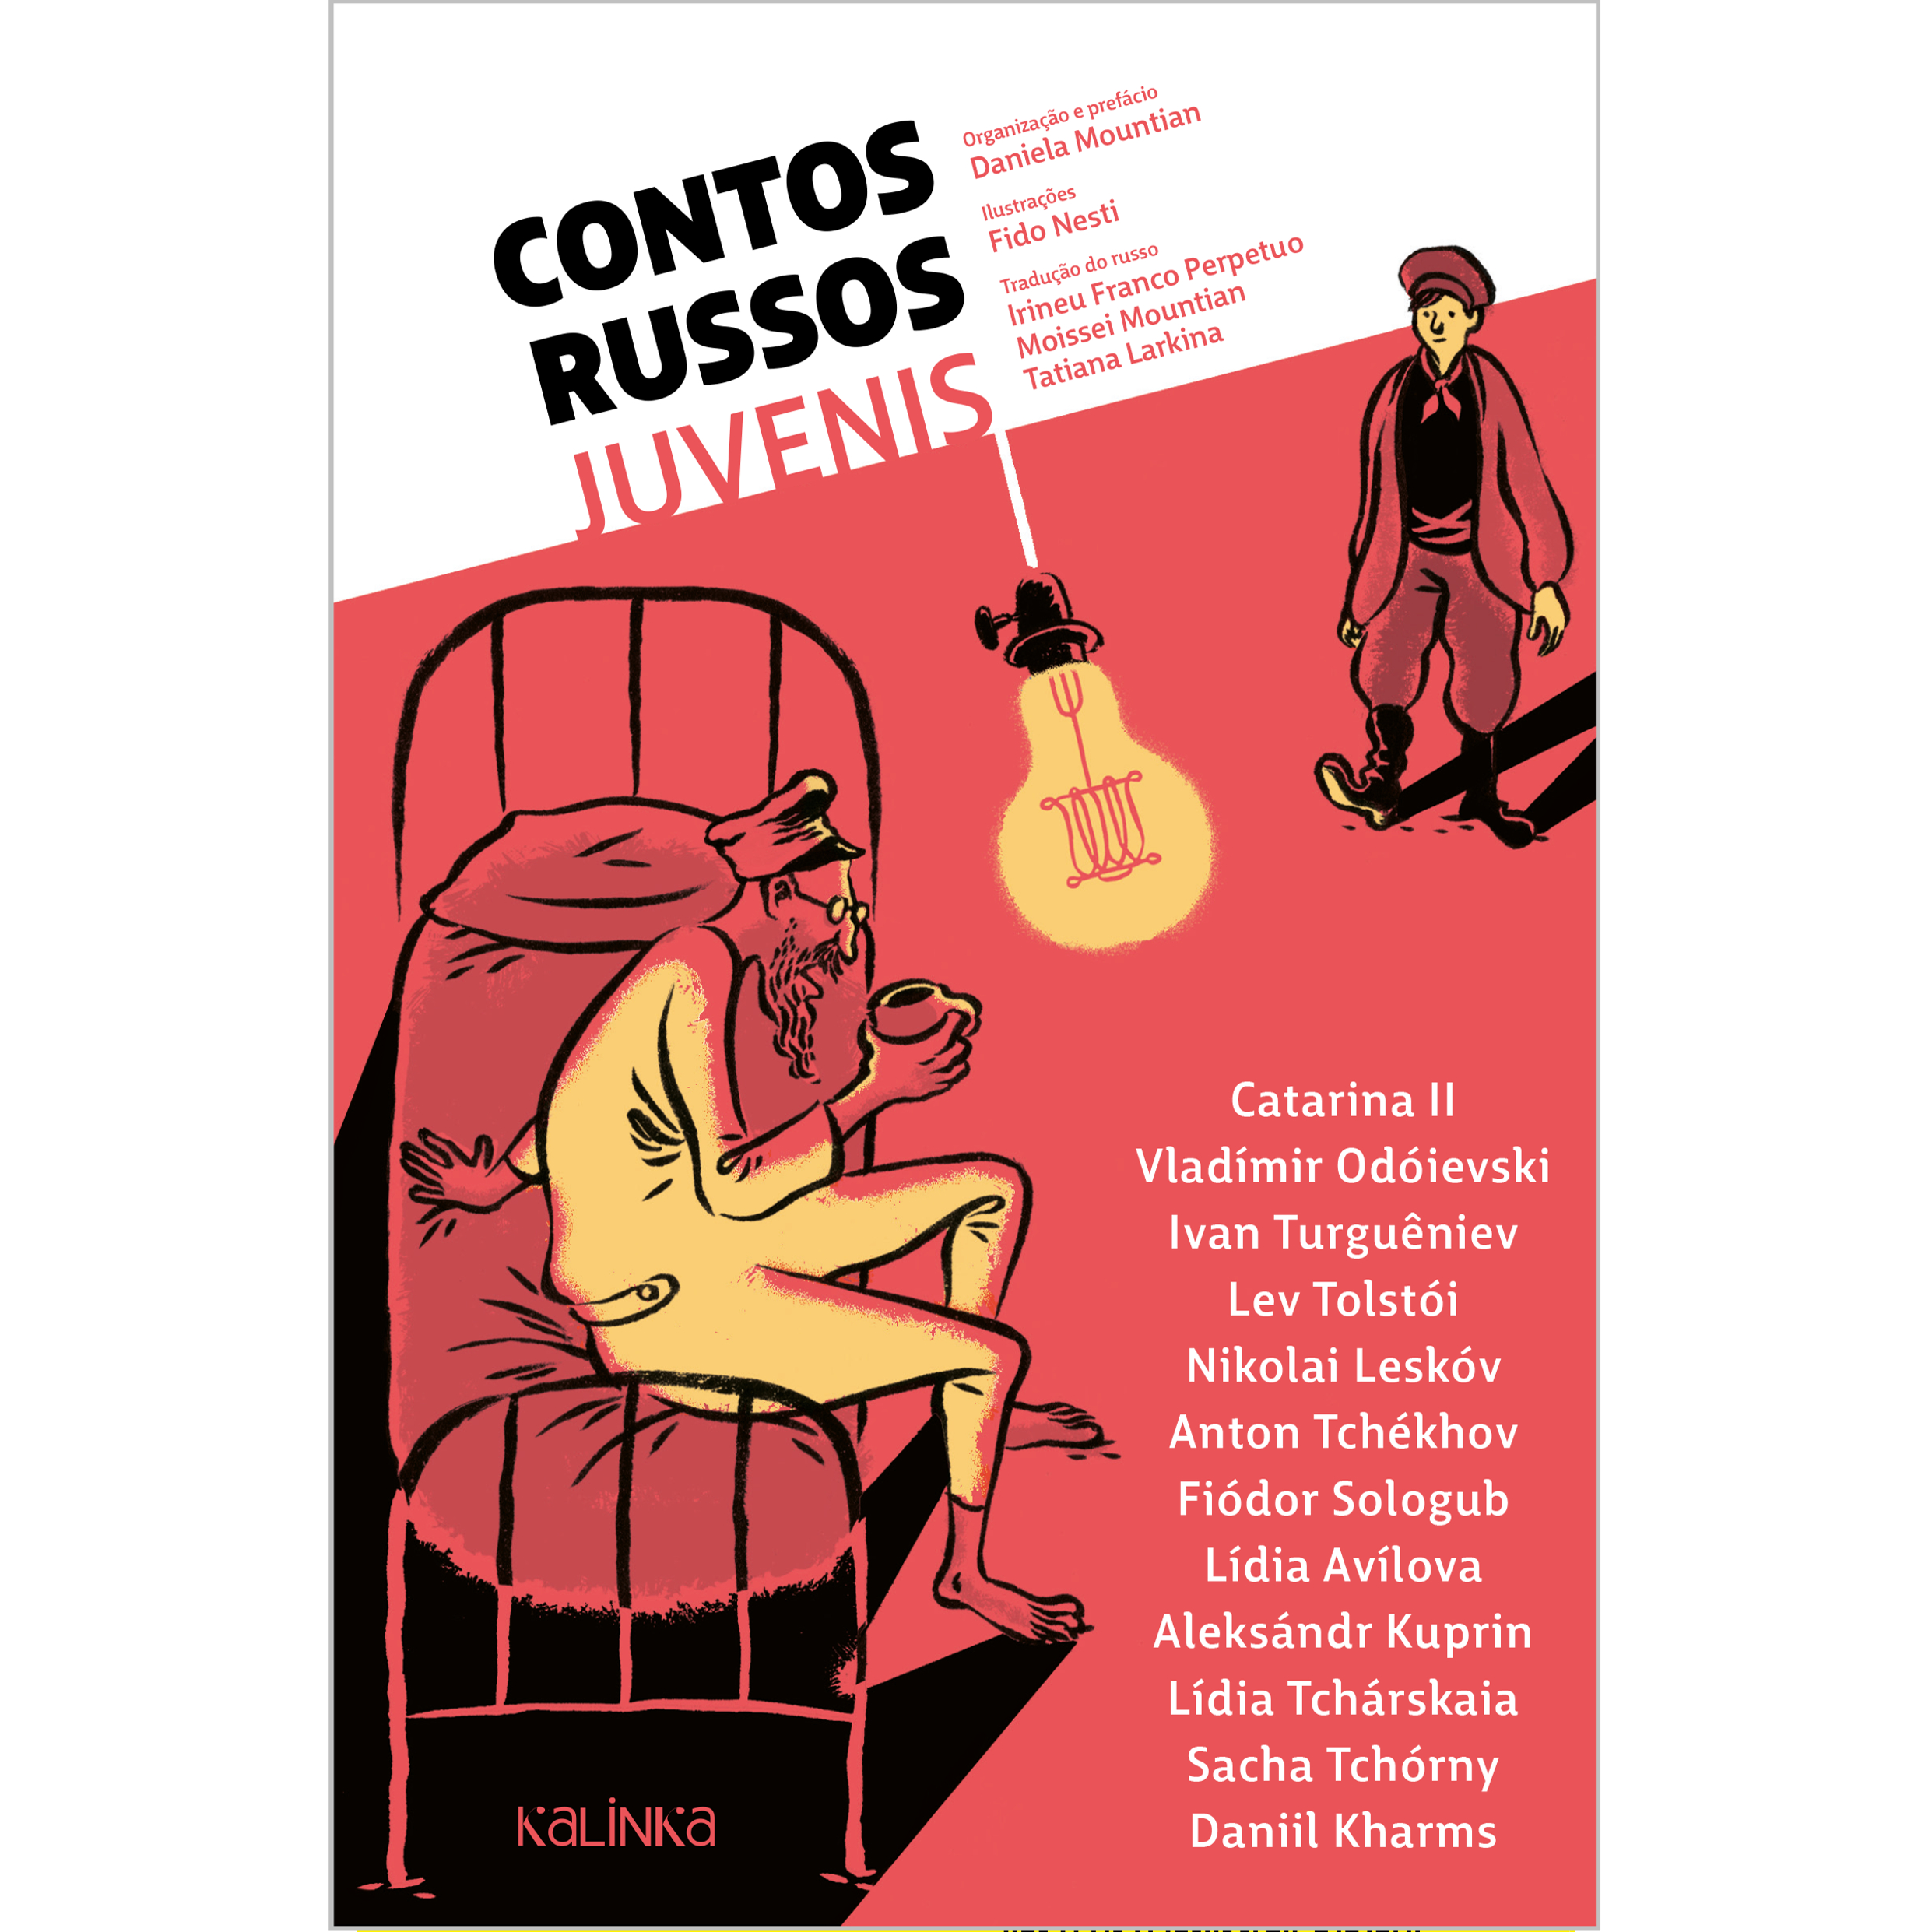
\includegraphics[width=74mm]{./grid/contos.jpg}
\end{center}

\hspace*{-7cm}\hrulefill\hspace*{-7cm}

\medskip

\noindent{}Esta coletânea reúne contos clássicos da literatura russa juvenil do fim do século \textsc{xviii} ao início do \textsc{xx}. A primeira escritora para os pequenos russos foi ninguém menos que Catarina \textsc{ii}. Nada mais historicamente justo do que começar nossa viagem por seu ``Conto do \textit{tsarévitche} Cloro'', que, com elementos universais e folclóricos, tornou-se um dos mais conhecidos textos da imperatriz. Seguindo a trilha dos contos populares, estão Nikolai Leskóv, com um relato embebido de cultura russa, e Fiódor Sologub, com um conto maravilhoso para jovens. Além de Anton Tchékhov e Lev Tolstói, autores lidos e relidos por gerações de russos, Lídia Avílova e Aleksándr Kuprin, que atentam ao universo infantil, e Lídia Tchárskaia, autora que mais causava sensação entre jovens russas do início do século \textsc{xx}. Também estão presentes Odóievski, Sacha Tchórny e Daniil Kharms, que anunciam o mundo contemporâneo com textos fantásticos, cheios de graça e humor. \hlc{As histórias nos fazem rir e chorar, nos levam para reinos distantes, para a costa da Crimeia, para as montanhas do Cáucaso, para as mais diversas paisagens imaginadas por artistas russos tão diversos quanto talentosos}.

\vfill

\hspace*{-.4cm}\begin{minipage}[c]{.5\linewidth}
\small\textbf{
\hspace*{-.1cm}Editora: Kalinka\\
Título: Contos russos juvenis\\
Autor: Daniela Mountian (org.)\\ 
ISBN: 978-65-86862-09-6\\
Páginas: 402\\
Formato: 14x21cm\\
Preço: R\$ 69,90
}
\end{minipage}

\pagebreak

\vspace*{1.5cm}

\noindent{}{\nohyphens{\LARGE{As crianças e a literatura russa}}}

\bigskip

\hfill{}\scalebox{.8}{DANIELA MOUNTIAN}

\bigskip
\bigskip
\bigskip

\begin{multicols}{2}
\noindent{}\lipsum[1]

\lipsum[2]

\lipsum[4]

\lipsum[6]


\noindent{}\textcolor{gray}{\footnotesize\slsc{Trecho da introdução do livro “Contos russos juvenis”.}}
\end{multicols}


\pagebreak 

\pagebreak
\pagestyle{kalinkacat}

\begin{multicols}{2}
\begin{enumerate}
\raggedright\nohyphens{
\item O compromisso, \textbf{Serguei Dovlátov}
\item Aulas de literatura russa: de Púchkin a Gorenstein, \textbf{Aurora Fornoni Bernardini}
\item O elefante, \textbf{Aleksandr Kuprin}
\item A velha, \textbf{Daniil Kharms}
\item Bobók \& Meia carta ``de um sujeito'', \textbf{Fiódor Dostoiévski}
\item Parque cultural, \textbf{Serguei Dovlátov}
\item O diabo mesquinho, \textbf{Fiódor Sologub}
\item Tarakã, o bigodudo, \textbf{Kornei Tchukóvski}
\item Salmo: romance-meditação sobre os quatro flagelos do senhor, \textbf{Friedrich Gorenstein}
\item O Ofício, \textbf{Serguei Dovlátov}
\item Luminescência: antologia poética, \textbf{Viatchesláv Kupriyánov}
\item Poesia russa: seleta bilíngue, \textbf{Vários}
\item Encontros com Liz e outras histórias, \textbf{Leonid Dobýtchin}
\item ``Os sonhos teus vão acabar contigo'': prosa, poesia, teatro, \textbf{Daniil Kharms}
\item A Cidade Ene, \textbf{Leonid Dobýtchin}
}
\end{enumerate}
\end{multicols}

\pagebreak




%\hspace{.5cm}
%
%\begin{center}
%\hspace*{-1cm}\raisebox{5.5cm}{\rotatebox[origin=t]{90}{\Formular{\textbf{Lançamento}}}}
%\hspace{1cm}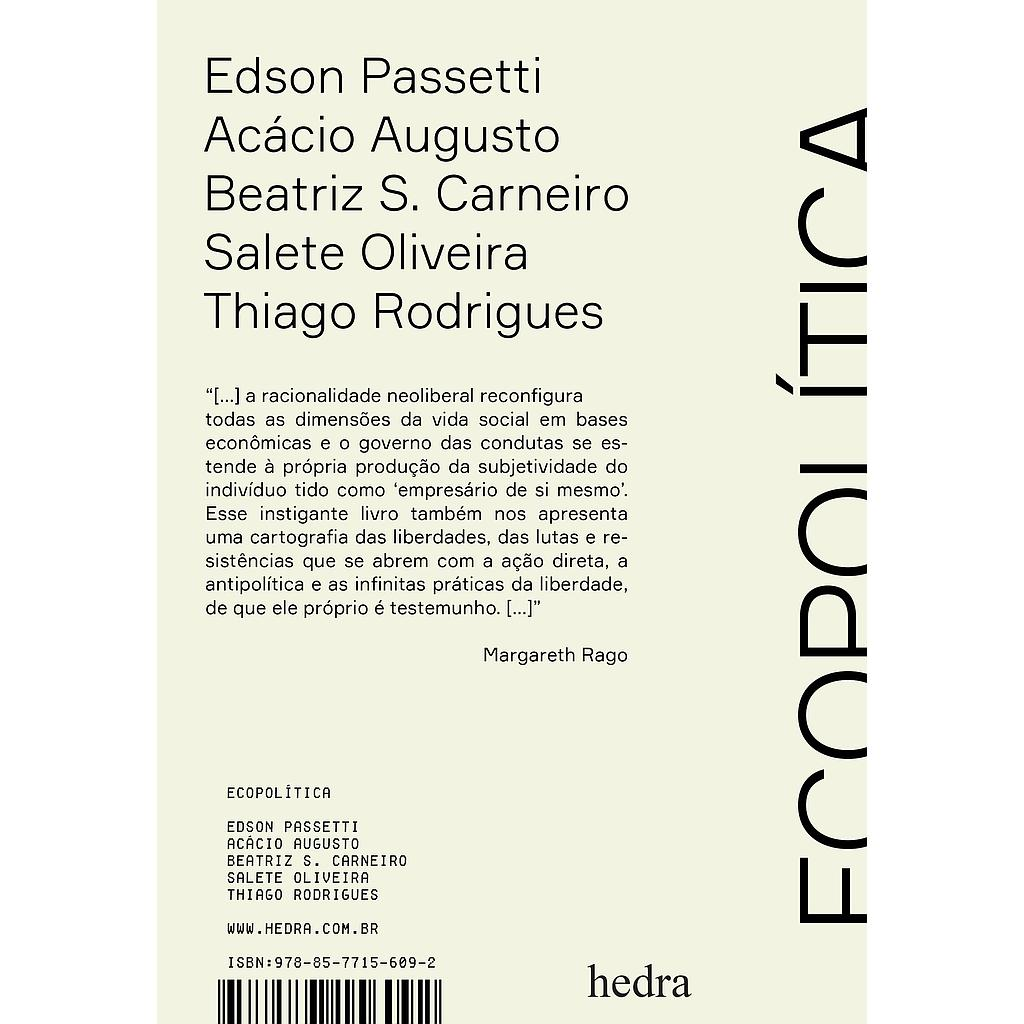
\includegraphics[width=70mm]{eco.jpeg}
%\end{center}
%
%\hspace*{-2cm}\_\_\_\_\_\_\_\_\_\_\_\_\_\_\_\_\_\_\_\_\_\_\_\_\_\_\_\_\_\_\_\_\_\_\_\_\_\_\%_\_\_\_\_\_\_\_\_\_\_\_\_\_\_\_\_\_\_\_\_\_\_\_\_\_\_\_\_\_\_\_\_\_\_\_
%
%\medskip
%
%\noindent{}Lorem ipsum dolor sit amet, consectetur adipiscing elit.
%Donec sodales tortor a purus accumsan, ut ultricies purus
%maximus. Aliquam bibendum consequat mi, sed commo-
%do velit pellentesque id. Vivamus ultricies ligula in semper
%sagittis. Donec mollis odio in lectus tristique, sed convallis
%est interdum. Cras eget sem condimentum, pretium purus
%eu, auctor.
%
%\hspace{.5cm}
%
%\hspace*{-.4cm}\begin{minipage}[c]{0.45\linewidth}
%\small{
%{\Formular{\textbf{
%\hspace*{-.1cm}Título: Ecopolítica\\
%Autor: Edson Passetti\\ 
%Editora: Hedra\\
%Páginas: 476\\
%Formato: 23x16cm\\
%Preço: R\$ 79,90\\
%}}}}
%\end{minipage}
%\begin{minipage}[c]{0.50\linewidth}
%\small{Lorem ipsum dolor sit amet, consectetur adipiscing elit. Donec sodales tortor a purus accumsan, ut ultricies. Lorem ipsum dolor sit amet, %consectetur adipiscing elit. Lorem ipsum dolor sit amet. Lorem ipsum dolor sit amet.} 
%\end{minipage}
%
%\pagebreak
%
%\hspace{.5cm}
%
%\begin{center}
%\hspace*{-.5cm}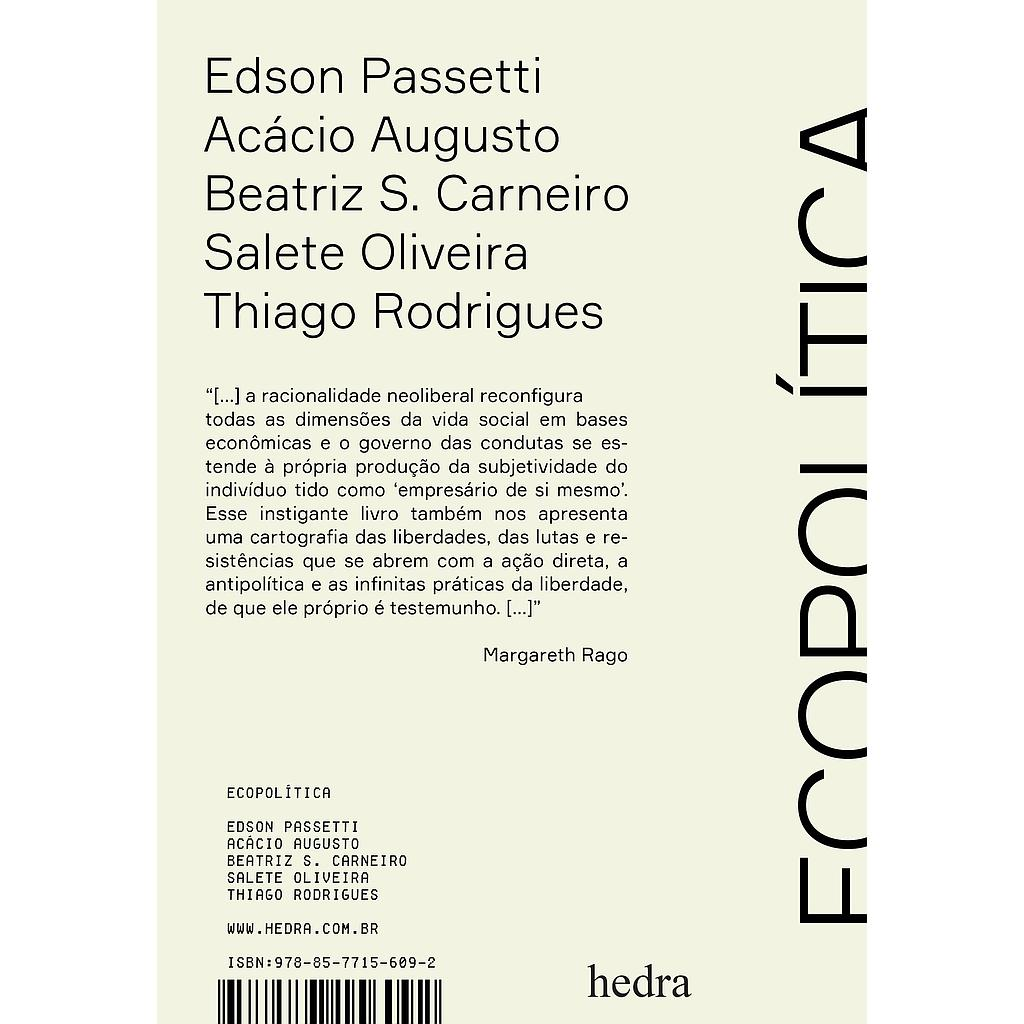
\includegraphics[width=70mm]{eco.jpeg}
%%\hspace*{6cm}\raisebox{2cm}{\rotatebox[origin=t]{90}{\Formular{\textbf{Lançamento}}}}
%\end{center}
%
%\hspace*{-2cm}\_\_\_\_\_\_\_\_\_\_\_\_\_\_\_\_\_\_\_\_\_\_\_\_\_\_\_\_\_\_\_\_\_\_\_\_\_\_\%_\_\_\_\_\_\_\_\_\_\_\_\_\_\_\_\_\_\_\_\_\_\_\_\_\_\_\_\_\_\_\_\_\_\_\_
%
%\medskip
%
%\noindent{}Lorem ipsum dolor sit amet, consectetur adipiscing elit.
%Donec sodales tortor a purus accumsan, ut ultricies purus
%maximus. Aliquam bibendum consequat mi, sed commo-
%do velit pellentesque id. Vivamus ultricies ligula in semper
%sagittis. Donec mollis odio in lectus tristique, sed convallis
%est interdum. Cras eget sem condimentum, pretium purus
%eu, auctor.
%
%\hspace{.5cm}
%
%\hspace*{-.4cm}\begin{minipage}[c]{0.45\linewidth}
%\small{
%{\Formular{\textbf{
%\hspace*{-.1cm}Título: Ecopolítica\\
%Autor: Edson Passetti\\ 
%Editora: Hedra\\
%Páginas: 476\\
%Formato: 23x16cm\\
%Preço: R\$ 79,90\\
%}}}}
%\end{minipage}
%\begin{minipage}[c]{0.50\linewidth}
%\small{Lorem ipsum dolor sit amet, consectetur adipiscing elit. Donec sodales tortor a purus accumsan, ut ultricies. Lorem ipsum dolor sit amet, %consectetur adipiscing elit. Lorem ipsum dolor sit amet. Lorem ipsum dolor sit amet.} 
%\end{minipage}
%
%\pagebreak